\section{Zakres projektu i harmonogram}

\subsection{Zakres}

\textbf{W zakresie projektu:}
\begin{itemize}
	\item przegląd metod detekcji tekstu AI (statystyka, ML, watermarking),
	\item wybór i przygotowanie zbioru danych (podział train/test, filtr długości),
	\item implementacja baseline'u opartego na cechach statystycznych,
	\item implementacja prostego modelu ML (o ile pozwolą dane),
	\item ewaluacja: dokładność oraz podstawowe metryki jakości klasyfikacji,
	\item porównanie wyników z ograniczeniami opisanymi w literaturze,
	\item dokumentacja wyników, ograniczeń i wniosków.
\end{itemize}

\textbf{Poza zakresem:}
\begin{itemize}
	\item detekcja w czasie rzeczywistym w produkcie komercyjnym,
	\item własne wdrażanie watermarkingu po stronie generatora,
	\item budowa lub hostowanie publicznego detektora znaków wodnych OpenAI (textGrain),
	\item pełna odporność na parafrazę, tłumaczenie i ataki adversarialne,
	\item gwarancja działania dla dowolnego języka i dowolnego modelu LLM,
	\item ocena prawna lub dowodowa wyniku detektora.
\end{itemize}

\subsection{Proponowane zbiory danych}

\begin{itemize}
	\item \textbf{LLM Detect AI Generated Text} (Kaggle) - gotowy zbiór do detekcji tekstu AI
	(\url{https://www.kaggle.com/datasets/sunilthite/llm-detect-ai-generated-text-dataset}).
	\item \textbf{SpeakLeash (Spichlerz)} - duży korpus tekstów polskich; źródło tekstów ludzkich do zestawu PL
	(\url{https://speakleash.org/}).
	\item \textbf{HC3 / M4} - zbiory badawcze (głównie EN): human vs ChatGPT / multi-generator.
	\item \textbf{AIDE} - eseje uczniowskie vs LLM (kontekst edukacyjny).
\end{itemize}

Na starcie planowane jest wykorzystanie zbioru z Kaggle oraz - w miarę możliwości - fragmentów SpeakLeash do eksperymentów z językiem polskim.

\subsection{Kamienie milowe}

\begin{enumerate}
	\item Zamknięcie przeglądu literatury i wymagań (październik 2026).
	\item Przygotowanie zbioru danych i pipeline'u ewaluacji (listopad 2026).
	\item Działający baseline statystyczny z wynikiem $\geq 51\%$ lub udokumentowaną przyczyną niepowodzenia (listopad--grudzień 2026).
	\item Opcjonalny model ML oraz porównanie z baseline'em (grudzień 2026).
	\item Sprawozdanie końcowe etapu z opisem ograniczeń (grudzień 2026).
\end{enumerate}

\subsection{Harmonogram (diagram Gantta)}

\begin{figure}[H]
\centering
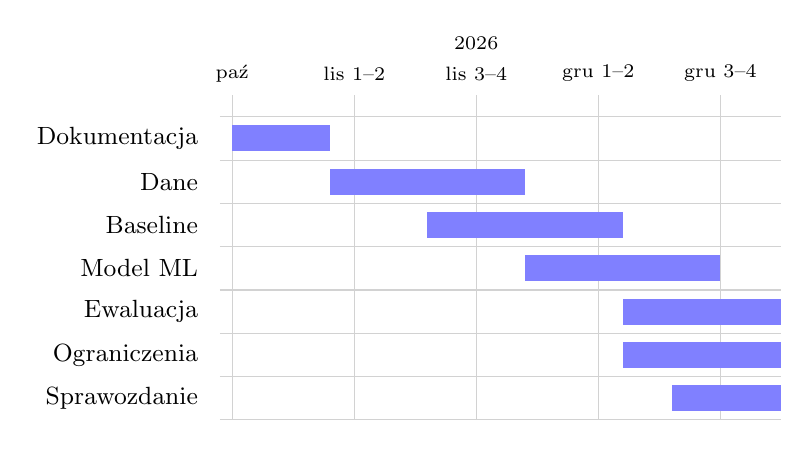
\begin{tikzpicture}[x=1.55cm,y=0.55cm]
\foreach \x/\lab in {0/paź,1/lis 1--2,2/lis 3--4,3/gru 1--2,4/gru 3--4}
  \node[font=\scriptsize] at (\x+2.6,8) {\lab};
\node[font=\scriptsize] at (4.6,8.7) {2026};
\foreach \y in {0,...,7}
  \draw[gray!35] (2.5,\y) -- (7.1,\y);
\foreach \x in {0,...,4}
  \draw[gray!35] (\x+2.6,0) -- (\x+2.6,7.5);
\fill[blue!50] (2.6,6.2) rectangle (3.4,6.8);
\node[anchor=east,font=\small] at (2.4,6.5) {Dokumentacja};
\fill[blue!50] (3.4,5.2) rectangle (5.0,5.8);
\node[anchor=east,font=\small] at (2.4,5.5) {Dane};
\fill[blue!50] (4.2,4.2) rectangle (5.8,4.8);
\node[anchor=east,font=\small] at (2.4,4.5) {Baseline};
\fill[blue!50] (5.0,3.2) rectangle (6.6,3.8);
\node[anchor=east,font=\small] at (2.4,3.5) {Model ML};
\fill[blue!50] (5.8,2.2) rectangle (7.1,2.8);
\node[anchor=east,font=\small] at (2.4,2.5) {Ewaluacja};
\fill[blue!50] (5.8,1.2) rectangle (7.1,1.8);
\node[anchor=east,font=\small] at (2.4,1.5) {Ograniczenia};
\fill[blue!50] (6.2,0.2) rectangle (7.1,0.8);
\node[anchor=east,font=\small] at (2.4,0.5) {Sprawozdanie};
\end{tikzpicture}
\caption{Orientacyjny harmonogram prac (październik - grudzień 2026)}
\end{figure}
